\chapter{脉搏波特征点检测及特征参数集的构建}
\section{引言}
前文已经阐述过,光电容积脉搏波(PPG)本身蕴含着丰富的血液动力学信息,其形态、强度、速率、节律等特征反映心脏的功能与状态,也可以反映出各级动脉及分支中血管壁弹性、血管阻力、血液黏度等信息。但同时,PPG信号也与其他医学电生理信号类似,
易收到多种噪声干扰。本章着重解决脉搏波信号的预处理问题与脉搏波描述等两个问题。前者主要涉及信号处理过程,后者则是寻找、挖掘、设计数字特征对量化描述脉搏波。最后,本章将多种脉搏波量化特征进行了汇总,构建了脉搏波一般描述特征集合。
\section{信号预处理}
:如何对原始信号脉搏波进行滤波降噪;如何

\subsection{信号滤波}

\subsection{波形检测及异常信号段处理}
脉搏波波形的正确检测是后续所有特征计算的基础,因此,如何
应用局部最大值原理

返回最大值所在位置


寻找峰值,寻找谷值,匹配


一、波形检测


二、异常信号处理


三、检测算法性能评估

\subsection{去除基线漂移}
在实际得到的PPG波形中,由于呼吸干扰等原因,一个完整PPG波形对应的两个波谷,即该波形的始末位置的幅值很难保持一致。这种差异最终会导致PPG信号的基线出现波动,也就是工程领域的基线漂移问题,如\autoref{fig:drift}所示。为满足后续特定PPG形态特征计算需求,
需要消除基线漂移的影响。此时一种基于线性变换的处理过程可以实现该目标。
\begin{figure}[htbp]
    \centering
    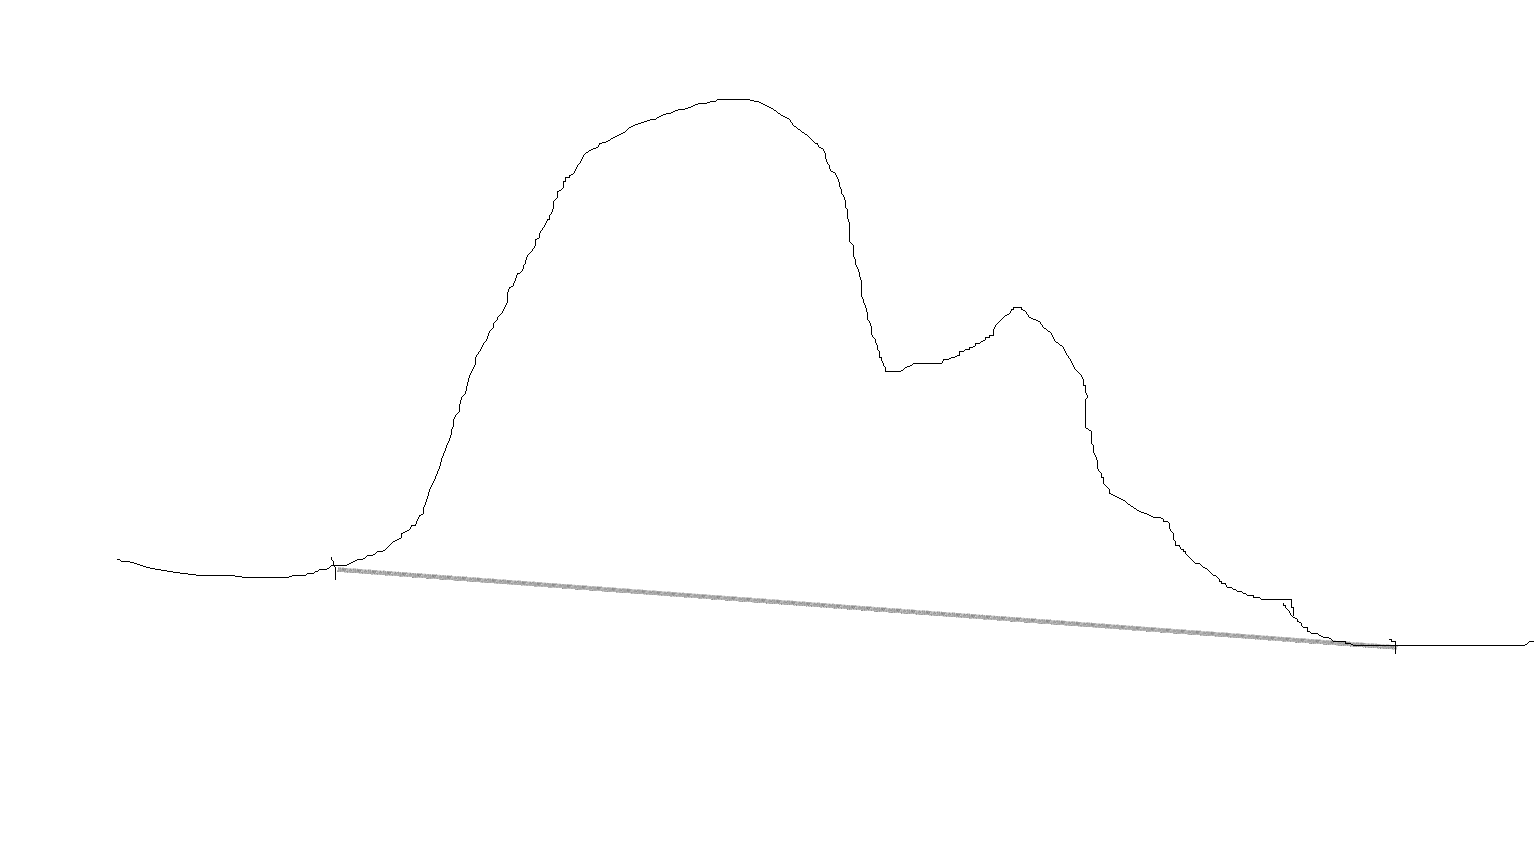
\includegraphics[width=.6\linewidth]{ch3/drift}
    \caption{\label{fig:drift}基线漂移去除示意及处理效果对比}
\end{figure}

如\autoref{fig:drift}所示,易知脉搏波的相对幅值$A$是采样时间$t$的函数,将其表示为$A(t)$。对任一特定波形,其起始点与终止点处对应的幅值可分别表示为$A(t_{start})$与$A(t_{end})$。
由于始末位置脉搏波幅值不等,则明显两者之间存在一条斜率不为0的直线,其具体值为
\begin{equation}
    \label{equ:linek}
    k=\frac{A(t_{start})-A(t_{end})}{t_{start}-t_{end}}
\end{equation}
则该直线上任意点即代表了在该时刻脉搏波波形与水平基线的偏移量,即
\begin{equation}
    \label{equ:liney}
    \Delta(t)=k(t-t_{start})+A(t_{start})
\end{equation}
此时,去除基线漂移后的脉搏波信号可标示为
\begin{equation}
    \label{equ:adjusta}
    A_{adjsut}(t)=A(t)-\Delta(t)
\end{equation}

\subsection{插值计算}
由于本章后部分自行定义设计的多种新型脉搏波特征,在特征计算过程中对脉搏波的采样频率有着较高要求。由于GE B450设备导出的原始脉搏波数据的采集频率仅为100$Hz$,难以满足后续计算。因此,需要在PPG预处理环节额外引入了插值计算操作以人工提高信号采样率。

插值是求值的逆过程,通过某些已知的数据点去推断一个(系列)特定的函数,使得所有已知数据点均在该函数图像上,从而去推断更多未知数据点,解决相应的实际问题,这一过程如\autoref{fig:spline}所示。
\begin{figure}[htbp]
    \centering
    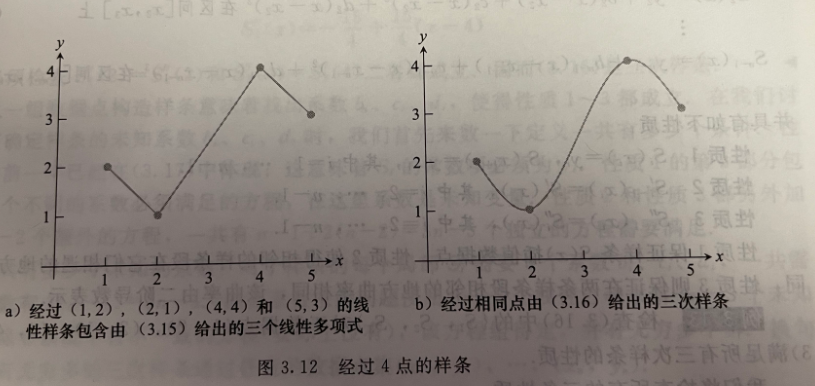
\includegraphics[width=.6\linewidth]{ch3/spline}
    \caption{\label{fig:spline}线性样条插值与三次样条插值对比}
\end{figure}
多项值插值与样条插值是插值最常用的两种算法\cite{Timothy2018,Carl2008}。多项式插值给出满足所有原始数据点的单一公式,由于此过程中仅涉及浮点数加法与乘法,因而得到广泛应用。而样条插值则使用多个公式,其中每个都是低阶多项式,来通过所有数据点。
其中,三次样条插值可以得到光滑的拟合插值曲线,在工业各领域中得到广泛应用。对原始数据点$(x_1,y_1),(x_1,y_1),\cdots,(x_n,y_n)$,三次样条的插值曲线$S(x)$在每两个数据分段区间$[x_i,x_{i+1}]$内均使用三阶多项式
\begin{equation}
    \label{equ:spline}
    S_{i}=y_{i}+b_{i}(x-x_{i})+c_{i}{(x-x_{i})}^2+d_{i}{(x-x_{i})}^3
\end{equation}
并保证每两个多项式在端点(即原始数据点)处不仅数值相等,相应的斜率与曲率均相等,即
\begin{equation}
    \label{equ:cubiccha}
    \left \{
    \begin{aligned}
        S_{i}(x_{i})&=y_i,&\text{i=1,$\cdots$,n-1}\\
        S_{i}(x_{i+1})&=y_{i+1},&\text{i=1,$\cdots$,n-1}\\
        S_{i}^{'}(x_{i-1})&=S_{i}^{'}(x_{i}),&\text{i=2,$\cdots$,n-1} \\
        S_{i}^{''}(x_{i-1})&=S_{i}^{''}(x_{i}),&\text{i=2,$\cdots$,n-1}
    \end{aligned}
    \right.
\end{equation}
使用微积分的定义,将\autoref{equ:spline}代入\autoref{equ:cubiccha}化简整理后,可以得到包含$3n-5$个独立方程的方程组。另一方面,由于每个局部$S_i$中有三个未知参数,一共有$3n-3$个待解参数,则此时由线性代数相关知识可知,该方程组有无穷多组解。
即此时可以构造处无穷多条通过所有数据点$(x_i,y_i)$的样条曲线。因此,需要添加额外的方程对样条曲线进行约束,一般的约束条件都是对样条左右端点处进行限定 ,常见的附加边界条件如\autoref{tab:splinekind}所示\cite{Timothy2018}。
\begin{table}[htbp]
    \centering
    \caption{\label{tab:splinekind}几种常见的三次样条端点条件}
    \begin{tabularx}{\linewidth}{X<{\centering}X<{\centering}}
        \toprule 
        \textbf{样条种类}&\textbf{端点条件}\\
        \midrule 
        自然三次样条&
        $
            S_{1}^{''}(x_{1})=0,
            S_{n-1}^{''}(x_{n})=0
        $
        \\
        曲率调整三次样条&
        $\left \{
        \begin{aligned}
            &S_{1}^{''}(x_{1})=v_1,&v_{1}\neq0\\
            &S_{n-1}^{''}(x_{n})=v_n,&v_{n}\neq0
        \end{aligned}
        \right.
        $
        \\
        钳制三次样条&
        $\left \{
        \begin{aligned}
            &S_{1}^{'}(x_{1})=v_1,&v_{1}\neq0\\
            &S_{n-1}^{'}(x_{n})=v_n,&v_{n}\neq0
        \end{aligned}
        \right.
        $
        \\
        抛物线端点三次样条&
        $
            d_1=0,d_{n-1}=0
        $
        \\
        非纽结三次样条&
        $
            d_1=d_2, d_{n-2}=d_{n-1}
        $
        \\
        \bottomrule
    \end{tabularx}
\end{table}

在补充\autoref{tab:splinekind}中的两个端点条件公式后,即可完成上述方程组求解,从而确定唯一的三次样条插值曲线。本研究中三次样条算法基于自然边界条件对PPG信号进行均匀插值\cite{ttk2021},使信号采样率被提高至2000$Hz$。
\subsection{数据标准化}

\section{脉搏波时域特征研究现状}
1. AIx

2. PWV

3. PSI

4. ADR

5. PTT

\section{时域特征参数设计与特征集构建}
\subsection{角度、幅值、长度等}
\section{小结}